\documentclass[conference]{IEEEtran}
\usepackage{amssymb,amsmath}
\usepackage{graphicx}
\usepackage{tabularx}
\usepackage{subfigure}
\usepackage{algorithm}
\usepackage{algorithmic}
\usepackage{epstopdf,mathrsfs}
\usepackage{hyperref}
\newtheorem{theorem}{Theorem}
\newtheorem{definition}{Definition}
\newtheorem{notation}{Notation}
\newtheorem{proposition}{Proposition}
\newtheorem{lemma}{Lemma}

\newcommand{\NP}{\mbox{${\cal NP}$}}

\begin{document}

\title{\LARGE Thermal-Constrained Energy-Aware Partitioning for Heterogeneous Multi-Core Multiprocessor Real-Time Systems}

\author{\IEEEauthorblockN{Shivashis Saha, Ying Lu, and Jitender S. Deogun}
\IEEEauthorblockA{Department of Computer Science and Engineering, \\
University of Nebraska-Lincoln,
Lincoln, NE 68588-0115, U.S.A. \\
Email: \{ssaha,ylu,deogun\}@cse.unl.edu} }


\maketitle


\begin{abstract}
Next-generation multi-core multiprocessor real-time systems consume less energy at the cost of increased power-density.
%Next-generation multi-core multiprocessor real-time systems consume less energy at the cost of increased power-density.
This increase in power-density results in high
heat-density and may affect the reliability and performance of real-time systems. Thus, incorporating maximum temperature
constraints in scheduling of real-time task sets is an important challenge.
This paper investigates thermal-constrained energy-aware %multi-core multiprocessor
partitioning of periodic real-time tasks in heterogeneous multi-core
multiprocessor systems. We adopt a power model which considers the impact of temperature and voltage on a processor's static power consumption.
Two types of thermal models are used to respectively capture negligible and non-negligible amount of heat
transfer among cores. %processors and cores.
We develop a novel genetic-algorithm based approach to solve the heterogeneous multi-core multiprocessor partitioning problem.
Extensive simulations were performed to validate the effectiveness of the approach.
Experimental results show that integrating a worst-fit based partitioning heuristic with the genetic algorithm %based approach
can significantly
reduce the  total energy consumption of a heterogeneous multi-core multiprocessor real-time system.
\end{abstract}

\vspace{-0.1in}

\section{Introduction}

An increased awareness for conserving energy has resulted in tremendous research interests in energy-efficient, %and
low-power design of computer systems \cite{Chen09}.
%The advances of
%Recent multiprocessor designs %architecture designs %lead to a
%translate into
%superior performance
%of multiprocessor systems over uniprocessor systems \cite{Chantem10}.
Next generation multiprocessor real-time systems are becoming
increasingly heterogeneous due to its relatively better performance and lower energy consumption compared to homogeneous counterparts~\cite{Kumar06}.
%The advances of multiprocessor architecture designs
%increase in power-density of multiprocessor systems has
However, energy efficiency of these recent multiprocessor systems comes at the cost of increased power-density.
This leads to  high heat-density which  in turn adversely affects the reliability and
performance of real-time systems \cite{Wang10}.
%The convex relationship between processor frequency and its power consumption has been
%exploited by \emph{dynamic voltage scaling} (DVS) techniques in real-time systems to minimize energy consumption \cite{Hong98}.


A processor's power consumption is composed of static and dynamic power consumptions. The static power consumption is
generated by the leakage current which is needed to maintain the activeness of the processor \cite{Chen09}. The dynamic power
consumption dissipated from executing a task on the processor
is a function of the processor's frequency \cite{Aydin03}. This function is assumed to be a strictly convex and monotonically increasing function,
which is usually represented by a polynomial of at least second degree \cite{Chen05}.
\emph{Dynamic voltage scaling} (DVS) techniques exploit the convex relationship to minimize the overall energy consumption \cite{Hong98}.
Energy-aware scheduling strategies for homogeneous multiprocessor systems using the DVS techniques and assuming negligible
leakage power consumption is well investigated  \cite{Chen07}. %in existing literature
However, the leakage current results in a significant static power consumption which is comparable to the dynamic power consumption \cite{Langen06}.
Leakage-aware partitioning strategies for heterogeneous systems were investigated recently in \cite{Chen09}, \cite{Langen09}.
The increase in the temperature of a processor due to an increased heat-density
%recent advances in semiconductor technologies
has resulted in a recent
research interest in temperature-aware multiprocessor scheduling
to improve the reliability and performance of homogeneous real-time systems \cite{Chantem10}, \cite{Quan10}, \cite{Fisher09}.
However, thermal-constrained energy-aware multiprocessor scheduling in heterogeneous real-time systems have not yet received much attention.

In this paper, we investigate thermal-constrained energy-aware partitioning-based scheduling of periodic tasks in heterogeneous multi-core multiprocessor real-time systems.
We consider a system which is heterogeneous across multiprocessors, but homogeneous within a multiprocessor.
Given a set of periodic tasks and a heterogeneous multi-core multiprocessor real-time system, the problem is to identify cores to be activated, allocate tasks to cores, and determine the frequencies of these cores such that the overall energy consumption is minimized, maximum temperature constraints are satisfied, and deadlines of all tasks are ensured.
%which leads to a minimum energy consumption while meeting deadlines of all tasks and satisfying temperature constraints of cores.
We consider a power model which captures not only the leakage power consumption \cite{Langen09}, but also the impact of  temperature \cite{Fisher09} and voltage \cite{Quan10} of a core on the leakage current.
We use two types of thermal models: \emph{heat-independent thermal (HIT) model}  --- negligible or no heat transfer
among cores \cite{Quan10}; and
\emph{heat-dependent thermal (HDT) model} --- non-negligible heat transfer among cores and sinks \cite{Chantem10}, \cite{Fisher09}.
We present a genetic-algorithm based approach to solve the heterogeneous multi-core multiprocessor partitioning problem.
Extensive simulations are performed to validate the effectiveness of the approach. Experimental data shows that the proposed algorithm,
HyWGA (\emph{Hybrid Worst-fit Genetic Algorithm}),
%HyWGA algorithm,
which integrates a Worst-fit based partitioning heuristic with the Genetic Algorithm, % \emph{Genetic Algorithm Based Scheduling Heuristic}
%and the \emph{Min-Core Worst-Fit Scheduling Heuristic} (MW heuristic)
is most effective in generating an allocation strategy that satisfies all the constraints and results in the minimum energy consumption.
The allocation strategy generated by HyWGA reduces the energy
consumption by up to 11\% and 21\% for HIT and HDT models respectively, as compared to the MW (\emph{Min-core Worst-fit}) heuristic.


\section{Related Work}

Extensive efforts have been made to study the multiprocessor real-time scheduling of periodic tasks~\cite{Carpenter04}.
In general, existing approaches can be categorized into two types: \emph{global} and \emph{partitioning-based} scheduling.
In the global scheduling~\cite{Baruah94}, all eligible tasks are assembled into a single queue,
from which the global scheduler selects tasks for execution.
%the highest priority tasks.
%in order of their priority.
On the contrary, the partitioning-based
approach allocates each task to a single processor, % on which each of its jobs executes,
and %thus
processors are scheduled independently~\cite{Baruah04}.
Due to simplicity in design and implementation, task partitioning approaches are more practical than global scheduling approaches \cite{Goraczko08}.
In this paper we focus on the partitioning approaches with the objective to make them energy-aware while satisfying thermal constraints.


Energy-aware %real-time
scheduling strategies for homogeneous multiprocessor systems have been extensively investigated~\cite{Chen07}.
%in existing literature
On the contrary, energy-aware scheduling strategies for heterogeneous multiprocessor systems have
received a limited attention \cite{Chen09}, where most of the work assumes a power model with a negligible leakage %power consumption
current \cite{Schranzhofer10}.
%Chen \emph{et. al} recently investigated
The impact of non-negligible, fixed leakage current on energy-aware scheduling for heterogeneous systems was only investigated recently \cite{Chen09}.
However, it has been proven that the leakage current of a processor changes super linearly with its temperature \cite{Liu07}. %, which was not considered in \cite{Chen09}.

Temperature-aware scheduling of real-time systems
has been investigated recently
%with the objective of satisfying the maximum temperature constraint \
\cite{Chantem10}, \cite{Quan10}, \cite{Fisher09}.
The authors of~\cite{Fisher09} and~\cite{Chantem10} respectively investigate scheduling sporadic and periodic tasks in
homogeneous multiprocessor systems to minimize %their
maximum temperatures.
The feasibility
checking problem for real-time periodic task sets under the maximum
temperature constraint was studied in \cite{Quan10}.
%However, t
The thermal models proposed
in \cite{Chantem10} and \cite{Fisher09}  capture   non-negligible %amounts of
heat  transfer between different
cores in a multi-core system. In these models, it was assumed that the leakage current is only impacted
by the temperature of the core \cite{Chantem10}, \cite{Fisher09}, \cite{Liu07}.
However, it has been %recently
proven that the leakage current is impacted not only by the temperature of a core, but also by its supply voltage \cite{Quan10}.

To the best of our knowledge, the thermal-constrained energy-aware
scheduling of periodic tasks in heterogeneous multi-core multiprocessor  systems has not yet received much attention. In this paper, we investigate partitioning-based scheduling %strategies
of periodic real-time tasks to minimize the total energy consumption, while satisfying maximum temperature constraints of
heterogeneous multi-core multiprocessor systems.
Our work is unique as we consider HIT \cite{Quan10} and HDT \cite{Chantem10}, \cite{Fisher09} thermal models to estimate the temperature of a processor, and use a power model
that captures the impact of both temperature \cite{Fisher09} and voltage \cite{Quan10} on a processor's static power consumption.
%We consider a power model which captures not only the impact of leakage current on the
%static power consumption \cite{Langen09}, but also captures the impact of  temperature \cite{Fisher09} and voltage \cite{Quan10} of a processor on the leakage current.
%We consider two types of thermal models to integrate both negligible \cite{Quan10} and non-negligible \cite{Chantem10}, \cite{Fisher09} amount of heat
%transfer among the cores during the
%estimation of the temperature of a processor.




\section{System Models and Problem Definition}
\label{sec:models}

%In this section we present the problem description, and the models used in this paper.

In this section, we describe our models and %define
the problem.
%the problem and its related models.

\subsection{Multiprocessor Model}

%We assume a set, $\Omega = \{\rho_1, \rho_2,\cdots, \rho_m\}$, of interconnected heterogeneous multiprocessor units. Each unit $\rho_i$ is
%assumed to have $k$ identical cores (or processors), i.e. $\rho_i = \{ \rho_{i,1}, \rho_{i,2}, \cdots, \rho_{i,k}\}$ ($i=1\ldots m$). A processor $\rho_{i,j}$
We consider a heterogeneous multiprocessor system, which is heterogeneous across multiprocessors, but homogeneous within a multiprocessor. That is, each multiprocessor may have different computational capacity, speeds/frequencies, and power and thermal parameters, but the cores within a given multiprocessor are homogeneous.
Let $\Omega = \{\rho_1, \rho_2,\cdots, \rho_m\}$ be a set of interconnected heterogeneous multiprocessor units, where
a unit $\rho_i$ has $k_i$ identical cores (or processors),
i.e. $\rho_i = \{ \rho_{i,1}, \rho_{i,2},$ $\cdots, \rho_{i,k_i}\}$ ($i=1\ldots m$), which can support dynamic voltage scaling (DVS) and vary its frequency to one of the discrete levels in the range
[$f^{min}_{i}$, $f^{max}_{i}$].
%Thus, our system is heterogeneous across multiprocessors, but homogeneous within a multiprocessor.
$f^{max}_{i}$ ($f^{min}_{i}$)  is the maximum (minimum) operating frequency of multiprocessor unit $\rho_i$.
For simple representation, we normalize the core frequency with respect to $f^{max}_{i}$.
A multiprocessor unit's throughput (or capacity) is assumed to be proportional to the normalized operating frequencies $f_{i,j}$ of its cores~\cite{Leping10}. The capacity of $\rho_i$, denoted by $\mu_i$, is
thus expressed as  $ \sum_{j=1}^{k_i} \alpha_i f_{i,j}$,
%expressed as Eq. \ref{eq:capacity},
where $\alpha_i$ is the performance coefficient of $\rho_i$.
In a heterogeneous multiprocessor system, higher values of $\alpha_i$ correspond to more powerful multiprocessor units.
 %(note that $\alpha_i$ makes the system heterogeneous across multiprocessors).
In the remainder of this paper, unless otherwise specified, frequency means normalized frequency.


%In our model, we assume each core has discrete frequencies, i.e. the
%operating frequency of each core is in the range of $[f^{min}_i , f^{max}_i]$ ($i=1\ldots m$) with a step size of $0.05$,
%where $f^{min}_i = 50\% f^{max}_i$.


%\begin{equation}\label{eq:capacity}
%\mu_i = \sum_{j=1}^{k} \alpha_i f_{i,j}
%\end{equation}

\subsection{Task Model}

Let  $\Gamma = \{\tau_1, \tau_2, \cdots, \tau_n\}$ be  a set of independent periodic real-time tasks.
%We assume a periodic real-time task set $\Gamma = \{T_1, T_2, \cdots, T_n\}$ that are independent in execution.
A periodic task $\tau_q$ is an infinite number of task instances (jobs) released with periodicity $P_q$ ($q=1\ldots n$)~\cite{Liu00}.
The period $P_q$ of a task $\tau_q$
also represents the relative deadline of the current job.
The worst-case execution time of $\tau_q$ is $W_q$ on a core of a standard multiprocessor $\wp$ with performance coefficient $\alpha_{\wp}=1$ and is
$\frac{W_q}{f}$ if the core has a constant frequency $f$.
Thus, task $\tau_q$'s worst-case utilization under the maximum frequency of a standard core is
$u_q = \frac{W_q}{P_q}$.
%, and its worst-case execution time on a core of a standard multiprocessor unit $\wp$ (whose performance coefficient $\alpha_{\wp}=1$) is  $W_i$.
%which
%This states that under a constant speed $S$, the worst-case execution time of running a job of $\tau_i$ on a standard uni-core processor is $\frac{W_i}{S}$. Thus, task $\tau_i$'s worst-case utilization under the maximum speed of a standard uni-core processor is $u_i = \frac{W_i}{P_i}$.
Let $U_{tot}$ denote the total
utilization of the task set $\Gamma$ under the maximum frequency of a standard core, i.e., $U_{tot} = \sum_{q=1}^{n} u_q = \sum_{q=1}^{n} \frac{W_q}{P_q}$.
A \emph{necessary} condition for a feasible schedule on the set $\Omega$ of multiprocessors is to have
$U_{tot} \leq  \sum_{i=1}^{m} k_i \alpha_i $, where $k_i$ and $\alpha_i$ as defined in Section~\ref{sec:models}-A denote the number of cores and the performance coefficient of multiprocessor unit $\rho_i$.
%given by Eq. \ref{eq:feasible},
%and thus we make this assumption throughout the paper.
We make this assumption throughout the paper.
%
%
%\begin{equation}\label{eq:feasible}
%%U_{tot} \leq \sum_{j=1}^{m} k \alpha_j %f_{max}^{j}
%%\mu_i = \sum_{j=1}^{k} \alpha_i f_{i,j}
%U_{tot} \leq  \sum_{j=1}^{m} k \alpha_j %f^{max}_{j}
%\end{equation}
%
%
In a partitioning-based multiprocessor system, given a task-to-processor partitioning, we can calculate the worst-case utilization $U_{i,j}$ of a core $\rho_{i,j}$ under its maximum frequency, i.e. $U_{i,j}=\frac{\sum_{\tau_r \in  \Gamma_{i,j}} W_r/P_r}{\alpha_i}=\frac{\sum_{\tau_r \in  \Gamma_{i,j}} u_r}{\alpha_i}$, where $\Gamma_{i,j}$ represents the set of tasks being allocated to $\rho_{i,j}$. Since each task is allocated to exactly one core, we have $U_{tot} = \sum_{q=1}^{n} u_q = \sum_{i=1}^{m} \sum_{j=1}^{k_i} \alpha_i U_{i,j}$.
We use $P$ to denote the hyper-period of task set $\Gamma$, i.e., the minimum positive number $P$ such that the released jobs are repeated every $P$ time units. For instance, $P$ is the least common multiple (LCM) of all task periods $P_1, \cdots, P_n$ when the periods are integral.
%Our problem focuses on the minimization of the overall energy consumption in the hyper-period $P$ while satisfying the maximum temperature constraint.
Thus, our objective is to minimize the overall energy consumption in the hyper-period $P$ while satisfying maximum temperature and real-time constraints.

\subsection{Power Model}
\label{power-model}

The power consumption of a core $\rho_{i,j}$  ($i=1\ldots m$, $j=1\ldots k_i$), denoted by $\Phi_{i,j}$ is composed of two
parts $\Phi^{s}_{i,j}$ and $\Phi^{d}_{i,j}$ (Eq. \ref{eq:tpower}). Here, $\Phi^{s}_{i,j}$ models the static
(or leakage) power consumption
generated by the leakage current required to maintain the activeness of the core \cite{Chen09,Langen06}, and
$\Phi^{d}_{i,j}$ models the dynamic power
consumption dissipated from executing a task on the core \cite{Aydin03}.
The static power consumption of a core $\rho_{i,j}$ denoted by  $\Phi^{s}_{i,j}$
is closely approximated  by Eq. \ref{eq:static} which models the dependence of leakage current on both the frequency $f_{i,j}$
\cite{Chantem10}, \cite{Fisher09} (proportional to the supply voltage \cite{Chaturvedi10})
and the temperature $T_{i,j}$ \cite{Quan10}, \cite{Chaturvedi10} of the core,
where $\gamma_i$ and $\delta_i$ are both non-negative constants dependent on the architecture of $\rho_i$. The dynamic power consumption of a core $\rho_{i,j}$ denoted by  $\Phi^{d}_{i,j}$
is a function of its frequency, i.e. $\Phi^{d}_{i,j} = g(f_{i,j})$.
In current DVS technologies, the function $g(f_{i,j})$ is assumed to be a strictly convex and monotonically increasing function,
which is usually represented by a polynomial of at least second degree.
As shown in Eq. \ref{eq:dynamic}, we assume that $\Phi^{d}_{i,j}$ is a cubic polynomial in frequency, i.e. involves $f_{i,j}^3$
\cite{Chantem10}, \cite{Quan10}, \cite{Fisher09}.
%where
$\chi_i$ is a non-negative constant
dependent on the architecture of $\rho_i$.

\vspace{-0.2in}

\begin{subequations}\label{eq:power}
	\begin{align}
		\Phi_{i,j}(f_{i,j}) &= \Phi^{s}_{i,j}(f_{i,j}) + \Phi^{d}_{i,j}(f_{i,j}) \label{eq:tpower} \\
		\Phi^{s}_{i,j}(f_{i,j}) &= \gamma_i f_{i,j} + \delta_i f_{i,j} T_{i,j} \label{eq:static}\\
		\Phi^{d}_{i,j}(f_{i,j}) &=  \chi_i  f_{i,j}^3 \label{eq:dynamic}
	\end{align}
\end{subequations}


\subsection{Temperature Model}

In this section, we present two different thermal models, % used in this paper,
namely \emph{heat-independent thermal model} \cite{Quan10} and \emph{heat-dependent thermal model} \cite{Chantem10}, \cite{Fisher09}.


%, there is heat transfer among the cores and sinks .

\subsubsection{Heat-Independent Thermal Model (HIT Model)}

\label{sec:simple}

%In this thermal model,
We assume there is negligible or no heat transfer among cores of a multiprocessor unit and among different units \cite{Quan10}, \cite{Chaturvedi10}.
Using the RC thermal model
\cite{Chen09}, \cite{Chantem10}, \cite{Quan10},  \cite{Fisher09}, \cite{Chaturvedi10}, %the equation of
the temperature of a core %,
%$\rho_{i,j}$  ($i=1\ldots m$, $j=1\ldots k$)
with respect to (wrt) time, %denoted by
$T_{i,j}(t)$ ($i=1\ldots m$, $j=1\ldots k_i$), %is formulated as
follows
Eq. \ref{eq:simple1}, where $T_i^{amb}$ is the ambient temperature (in $^\circ C)$,
$R_i$ is the thermal resistance (in $J/ ^\circ C)$, and $C_i$ is the thermal capacitance (in $Watt/ ^\circ C)$ of $\rho_i$; $\Phi_{i,j}(t)$ is the power consumption of core $\rho_{i,j}$  wrt time (in $Watt)$,
and $\frac{dT_{i,j}(t)}{dt}$ is the derivative of $\rho_{i,j}$'s  temperature wrt time.


\vspace{-0.1in}

\begin{equation}\label{eq:simple1}
R_iC_i\frac{dT_{i,j}(t)}{dt} + T_{i,j}(t) - R_i\Phi_{i,j}(t) = T_i^{amb}
\end{equation}

\vspace{-0.1in}

Let the initial temperature of $\rho_{i,j}$  at time $t_0$ be $T^{0}_{i,j}$. If $\rho_{i,j}$  is running at a constant frequency $f_{i,j}$,
then its final temperature at time $t_1$,  denoted by $T^{1}_{i,j}$, is given by Eq. \ref{eq:final_simple}.
%The values of $T^{0}_{i,j}$ and $T^{1}_{i,j}$ are scaled such that $T_i^{amb}=0$ \cite{Quan10}, \cite{Chaturvedi10}.


\begin{subequations} \label{eq:final_simple}
\vspace{-0.1in}
	\begin{equation}
		\frac{dT_{i,j}}{dt} = \frac{T_i^{amb} + \gamma_i R_i f_{i,j} + \delta_i R_i f_{i,j} T_{i,j} +  \chi_i R_i f_{i,j}^3}{R_iC_i} - \frac{T_{i,j}}{R_iC_i}
	\end{equation}

	\vspace{-0.2in}

	\begin{equation}
		\int_{T^{0}_{i,j}}^{T^{1}_{i,j}} \frac{dT_{i,j}}{ \frac{ T_i^{amb} + \gamma_i R_i f_{i,j} + \chi_i R_i f_{i,j}^3}{R_iC_i} - (  %\frac{1}{R_iC_i} -
		\frac{1 - \delta_i R_i f_{i,j}}{R_iC_i} ) T_{i,j}}   = \int_{t_0}^{t_1} dt
	\end{equation}

	\vspace{-0.2in}
\footnotesize
	\begin{equation}
	\begin{split}
		T^{1}_{i,j} &= \frac{\frac{T_i^{amb} + \gamma_i R_i f_{i,j} + \chi_i R_i f_{i,j}^3}{R_iC_i}}{\frac{1 - \delta_i R_i f_{i,j}}{R_iC_i}} \; \; -  \\
		&\quad \left(\frac{\frac{T_i^{amb} + \gamma_i R_i f_{i,j} + \chi_i R_i f_{i,j}^3}{R_iC_i} }{\frac{1 - \delta_i R_i f_{i,j}}{R_iC_i}}
		- T^{0}_{i,j} \right) e ^{- ( \frac{1 - \delta_i  R_i f_{i,j}}{R_iC_i})(t_1 - t_0)}
	\end{split}
	\end{equation}

	\vspace{-0.2in}
	\begin{equation}
	\begin{split}
		T^{1}_{i,j} &= \frac{T_i^{amb} + \gamma_i R_if_{i,j} + \chi_i R_if_{i,j}^3}{1-\delta_i R_if_{i,j}} \; \;- \\
		&\quad \left( \frac{T_i^{amb} +  \gamma_i R_if_{i,j} +
		\chi_i R_if_{i,j}^3}{1-\delta_i R_if_{i,j}} -
		T^{0}_{i,j}  \right) e^{- (\frac{1 - \delta_i R_if_{i,j}}{R_iC_i}) (t_1 - t_0)}
	\end{split}
	\end{equation}
\end{subequations}


The temperature of $\rho_{i,j}$  is a non-decreasing function as long as it runs at a constant frequency (Eq. \ref{eq:final_simple})
\cite{Chantem10}, \cite{Quan10}, \cite{Fisher09},  \cite{Chaturvedi10}.
It will become steady when the system reaches a steady state condition $\left(\frac{dT_{i,j}(t)}{dt}=0\right)$.  The maximum temperature of the
core running at constant frequency $f_{i,j}$ is denoted by $T^*_{i,j}$ $ \left(\frac{d^2T_{i,j}(t)}{dt^2} \arrowvert_{T_{i,j}(t)=T^*_{i,j}} >0\right)$.
%The value of $T^*_{i,j}$ %(assuming $T_{amb}=0$)
%is given by Eq. \ref{eq:max1}.
$T^*_{i,j}$ is estimated using Eq. \ref{eq:max1}.

\vspace{-0.1in}

\begin{equation}\label{eq:max1}
%\begin{split}
			0 =  \frac{ T_i^{amb} + \gamma_i  R_i f_{i,j} + \delta_i  R_i f_{i,j} T^*_{i,j} + \chi_i  R_i f_{i,j}^3 } { R_iC_i} - \frac{T^*_{i,j}}{R_iC_i}
\end{equation}

\vspace{-0.1in}

Simplifying Eq. \ref{eq:max1}, we get Eq. \ref{eq:peak1}

\vspace{-0.1in}

\begin{equation}\label{eq:peak1}
T^*_{i,j} = \frac{ \frac{T_i^{amb} + \gamma_i R_i f_{i,j} + \chi_i R_i f_{i,j}^3}{R_iC_i} }{ \frac{1 - \delta_iR_i f_{i,j}}{R_iC_i} } =
\frac{T_i^{amb} + \gamma_i R_if_{i,j} + \chi_i R_if_{i,j}^3}{1-\delta_i R_if_{i,j}}
\end{equation}
\vspace{-0.2in}


\subsubsection{Heat-Dependent Thermal Model (HDT model)}
\label{sec:complex}

%In this thermal model,
We assume there is non-negligible heat transfer among cores of a multiprocessor unit \cite{Chantem10}, \cite{Fisher09}.
We also assume that there is negligible or no heat transfer among different multiprocessor units.
In a multiprocessor unit $\rho_i$ ($i=1\ldots m$), we assume there is a set of heat sinks, $\Xi_i = \{\varpi_{i,1}, \varpi_{i,2},\cdots, \varpi_{i,h_i}\}$.
These heat sinks are placed on top of the cores, and are only used for heat dissipation. These heat sinks do not generate any power.
The transfer of heat among the cores and heat sinks of a multiprocessor unit can be closely approximated by modeling
the dynamic heat transfer process
using Fourier's Law, where
each core acts as a discrete thermal element  \cite{Chantem10}, \cite{Fisher09}.


Using RC thermal model \cite{Chantem10}, \cite{Fisher09}, we assume the thermal conductance between two cores $\rho_{i,j}$ and $\rho_{i,j'}$ is
$\omega^{i}_{j,j'} (\forall j,j' \in 1\ldots k_i$). %; \rho_{i,j}$ and $\rho_{i,j'}$ has intersection for heat transfer).
%If $\rho_{i,j}$ and $\rho_{i,j'}$  has no intersection for heat transfer, then $\omega^{i}_{j,j'}=0$.
Let $\zeta^{i}_{j,q}$ represent the vertical thermal conductance
between core $\rho_{i,j}$ and sink $\varpi_{i,q}$ ($q=1\ldots h_i$), and $\omega^{i}_{q,q'}$ be the horizontal thermal conductance between
the heat sinks ($\forall q,q' \in 1\ldots h_i$).
%If $\rho_{i,j}$ and $\varpi_{i,q}$ has no heat transfer, then $\zeta^{i}_{j,q}=0$.
We assume that $\omega^{i}_{j,j'}$=$\omega^{i}_{j',j}$, $\omega^{i}_{j,j}$=$0$, $\omega^{i}_{q,q'}$=$\omega^{i}_{q',q}$, and
$\omega^{i}_{q,q}$=$0$. The thermal conductance between the heat sink and the environment is denoted by $\omega_i^{amb}$.
The thermal capacitance of $\rho_i$ and $\Xi_i$ are denoted by $C_i$ and $C^{sink}_i$ respectively.
The equation of $\rho_{i,j}$'s temperature wrt time, $T_{i,j}(t)$, is formulated as  Eq. \ref{eq:complex1}.
In  Eq. \ref{eq:complex1}, $\frac{dT_{i,j}(t)}{dt}$ is the derivative of $\rho_{i,j}$'s  temperature wrt time, and
$\Phi_{i,j}(t)$ is $\rho_{i,j}$'s power consumption wrt time.
Similarly, the equation of $\varpi_{i,q}$'s temperature wrt time, denoted by $T^{sink}_{i,q}(t)$, is formulated as  Eq. \ref{eq:complex2}.
In  Eq. \ref{eq:complex2}, $\frac{dT^{sink}_{i,q}(t)}{dt}$ is the derivative of $\varpi_{i,q}$'s temperature wrt time, and
$T_i^{amb}$ is the ambient temperature.


\vspace{-0.2in}

\begin{equation}\label{eq:complex1}
\footnotesize
\begin{split}
	C_i \frac{dT_{i,j}(t)}{dt} &= \Phi_{i,j}(t) - \sum_{j'=1}^{k_i} \omega^{i}_{j,j'} ( T_{i,j}(t) - T_{i,j'}(t) ) \\
	&\quad  - \sum_{q=1}^{h_i} \zeta^{i}_{j,q} ( T_{i,j}(t) - T^{sink}_{i,q}(t) )
\end{split}
\end{equation}

\vspace{-0.23in}

\begin{equation}\label{eq:complex2}
\footnotesize
\begin{split}
	&C^{sink}_i \frac{dT^{sink}_{i,q}(t)}{dt} = - \omega_i^{amb} (T_{i,q}^{sink}(t) - T_i^{amb}) \\
 	&\quad - \sum_{j=1}^{k_i} \zeta^{i}_{j,q} (T^{sink}_{i,q}(t) - T_{i,j}(t)) %\\
	 	%&\quad
	 	- \sum_{q'=1}^{h_i} \omega^{i}_{q,q'} (T^{sink}_{i,q}(t) - T^{sink}_{i,q'}(t) )
\end{split}
\end{equation}


\vspace{-0.1in}

The temperature of $\rho_{i,j}$  is a non-decreasing function as long as it runs at a constant frequency
\cite{Chantem10}, \cite{Quan10}, \cite{Fisher09},  \cite{Chaturvedi10}.
It will become steady when the system reaches a steady state condition $\left(\frac{dT_{i,j}(t)}{dt}=0, \frac{dT^{sink}_{i,q}(t)}{dt}=0\right)$.
The maximum temperature of the
core running at constant frequency $f_{i,j}$ is denoted by $T^*_{i,j}$ $ \left(\frac{d^2T_{i,j}(t)}{dt^2} \arrowvert_{T_{i,j}(t)=T^*_{i,j}} >0\right)$,
and the maximum temperature of the heat sink $\varpi_{i,q}$ is denoted by $T^{sink*}_{i,q}$ $ \left(\frac{d^2T^{sink}_{i,q}(t)}{dt^2} \arrowvert_{T^{sink}_{i,q}(t)=T^{sink*}_{i,q}} >0\right)$. The values of $T^*_{i,j}$ and  $T^{sink*}_{i,q}$ are given by Eq. \ref{eq:complex_max1}

\vspace{-0.2in}

\begin{subequations} \label{eq:complex_max1}
	\begin{equation}
		\begin{split}
			0 &= ( \gamma_i f_{i,j} + \delta_i f_{i,j} T^*_{i,j} + \chi_i  f_{i,j}^3 )
			 	- \sum_{j'=1}^{k_i} \omega^{i}_{j,j'} ( T^*_{i,j} - T^*_{i,j'} ) \\
			&\quad  - \sum_{q=1}^{h_i} \zeta^{i}_{j,q} ( T^*_{i,j} - T^{sink*}_{i,q} ) \\
			&= (\gamma_i f_{i,j} + \chi_i  f_{i,j}^3 ) + T^*_{i,j} \left( \delta_i f_{i,j} - \sum_{j'=1}^{k_i} \omega^{i}_{j,j'} - \sum_{q=1}^{h_i} \zeta^{i}_{j,q} \right) \\
			&\quad + \sum_{j'=1}^{k_i} \omega^{i}_{j,j'} T^*_{i,j'} + \sum_{q=1}^{h_i} \zeta^{i}_{j,q} T^{sink*}_{i,q}
		\end{split}
	\end{equation}

\vspace{-0.2in}

	\begin{equation}
		\begin{split}
			0 &= - \omega_i^{amb} (T_{i,q}^{sink*} - T_i^{amb}) - \sum_{j=1}^{k_i} \zeta^{i}_{j,q} (T^{sink*}_{i,q} - T^*_{i,j}) \\
			&\quad - \sum_{q'=1}^{h_i} \omega^{i}_{q,q'} (T^{sink*}_{i,q} - T^{sink*}_{i,q'} ) \\
			&= \omega_i^{amb} T_i^{amb} + T^{sink*}_{i,q} \left( - \omega_i^{amb} -\sum_{j=1}^{k_i} \zeta^{i}_{j,q} - \sum_{q'=1}^{h_i} \omega^{i}_{q,q'} \right ) \\
			&\quad + \sum_{j=1}^{k_i} \zeta^{i}_{j,q} T^*_{i,j} + \sum_{q'=1}^{h_i} \omega^{i}_{q,q'}  T^{sink*}_{i,q'}
		\end{split}
	\end{equation}
\end{subequations}

\vspace{-0.2in}

Simplifying Eq. \ref{eq:complex_max1} we get Eq. \ref{eq:complex_peak1} \cite{Fisher09}, where %with the following notations

\vspace{-0.2in}


\begin{equation*}
	\begin{split}
	A_{j,j} & = \delta_i f_{i,j} - \sum_{j'=1}^{k_i} \omega^{i}_{j,j'} - \sum_{q=1}^{h_i} \zeta^{i}_{j,q} \\
	A_{j,j'} &=  \omega^{i}_{j,j'} \\
	A_{j,k_i+q} &= A_{k_i+q,j} = \zeta^{i}_{j,q} \\
	A_{k_i+q,k_i+q} &=  - \omega_i^{amb} -\sum_{j=1}^{k_i} \zeta^{i}_{j,q} - \sum_{q'=1}^{h_i} \omega^{i}_{q,q'} \\
	A_{k_i+q,k_i+q'} &= \omega^{i}_{q,q'}
	\end{split}
\end{equation*}

\vspace{-0.2in}

\begin{subequations} \label{eq:complex_peak1}
%\footnotesize
\scriptsize
	\begin{equation} \label{eq:mat}
	%\begin{split}
		\begin{pmatrix}
		A_{1,1} & \ldots & A_{1,k_i+h_i} \\
		\vdots & \vdots & \vdots \\
		A_{k_i,1} & \ldots & A_{k_i, k_i+h_i} \\
		A_{k_i+1, 1} & \ldots & A_{k_i+1, k_i+h_i} \\
		\vdots & \vdots & \vdots \\
		A_{k_i+h_i, 1} & \ldots & A_{k_i+h_i,k_i+h_i}
		\end{pmatrix}
		\begin{pmatrix}
		T^*_{i,1} \\
		\vdots \\
		T^*_{i,k_i}  \\
		T^{sink*}_{i,k_i+1}  \\
		\vdots \\
		T^{sink*}_{i,k_i+h_i}
		\end{pmatrix}
		= - \begin{pmatrix}
		\gamma_i f_{i,1} + \chi_i  f_{i,1}^3  \\
		\vdots \\
		\gamma_i f_{i,k_i} + \chi_i  f_{i,k_i}^3   \\
		\omega_i^{amb} T_i^{amb}  \\
		\vdots \\
		\omega_i^{amb} T_i^{amb}
		\end{pmatrix}
	%\end{split}
	\end{equation}

%\vspace{-0.2in}
\normalsize

%\text{We denote Eq. \ref{eq:complex_peak1} by}

\vspace{-0.2in}

	\begin{equation}
	\text{We denote Eq. \ref{eq:mat} by} ~~ \left[A\right]_{k_i+h_i,k_i+h_i} \times \left[T\right]_{k_i+h_i,1} = - \left[\lambda\right]_{k_i+h_i,1}
	\end{equation}

\vspace{-0.2in}

%\vspace{-0.2in}

	\begin{equation}
	\text{Thus,} ~~ \left[T\right]_{k_i+h_i,1} = - \left[A\right]^{-1}_{k_i+h_i,k_i+h_i} \times \left[\lambda\right]_{k_i+h_i,1}
	\end{equation}
\end{subequations}

\subsection{Problem Definition}
\label{sec:pd}

Consider a core of a multiprocessor unit, $\rho_{i,j}$, and a set of periodic real-time tasks allocated to the core whose utilizations sum up to $U$, satisfying $U \leq \alpha_i$. That is, the set of tasks' utilization on core $\rho_{i,j}$ is $U_{i,j} = \frac{U}{\alpha_i} \leq 1$.
%
%\begin{proposition} \label{prop1}
%Consider a uni-core multiprocessor unit $\rho_i$, and a set of periodic real-time tasks allocated to $\rho_i$ whose total utilization satisfies $U_{tot} \leq \alpha_i$. The speed of the core needed to minimize the total energy consumption while meeting all deadlines is constant (denoted by $\overline{f_i}$) and is equal to $\overline{f_i} = U_{tot}$. Moreover, when the core is used along with this speed $\overline{f_i}$, any periodic hard real-time scheduling policy which can fully utilize the core (e.g., Earliest Deadline First (EDF)) can be used to obtain a feasible schedule \cite{Aydin01}.
%\end{proposition}
%
According to the work by Aydin et al.~\cite{Aydin01}, if we make the frequency of a core to be at least $U_{i,j}$, any periodic hard real-time scheduling policy which can fully utilize the core (e.g., Earliest Deadline First, Least Laxity First) can be used to obtain a feasible schedule.
We therefore assume that core $\rho_{i,j}$ ($i=1 \ldots m, j=1 \ldots k_i$) chooses a frequency $\tilde{f}_{i,j}$ , which is the lowest discrete frequency  greater than or equal to $U_{i,j}$. Then, core $\rho_{i,j}$'s energy consumption  $P \times \Phi_{i,j}(\tilde{f}_{i,j})$ in the interval $[0,P]$ can be estimated using Eq. \ref{eq:power}.
$T^{max}_{i,j}$ is the maximum allowed operating temperature of $\rho_{i,j}$.
Since the system will eventually reach  steady state with maximum temperature $T^*_{i,j}$, we need to make sure that setting $\rho_{i,j}$'s frequency at $\tilde{f}_{i,j}$, $T^*_{i,j}$ is no greater than $T^{max}_{i,j}$.

\subsubsection{Problem Statement}

Given a set of periodic real-time tasks ($\Gamma$), and a set of interconnected heterogeneous multi-core multiprocessor units ($\Omega)$,
%The problem is to partition the real-time tasks for minimizing the overall energy consumption while meeting all deadlines.
the problem is to identify the cores to be activated, allocate tasks to these active cores, and determine the frequencies of these cores
such that the overall energy consumption is minimized, maximum temperature constraints are satisfied, and deadlines of all tasks are ensured. We assume that inactive cores can be turned off. % (i.e. speed of inactive core is zero).
%Thus, our objective is to find an energy-optimal partitioning of the real-time tasks while meeting all the deadlines and satisfying the maximum temperature constraints of the multiprocessors.
This problem is known to be $\NP$-Hard in the strong sense \cite{Aydin03}, \cite{Stankovic95}.
We state the problem as follows, where $\Psi$ and $c_i$ respectively represent the set of active multiprocessors and
%where $l$ and $c_i$ respectively represent the number of active multiprocessor units and
the number of active cores in $\rho_i$. % $(i=1 \ldots m)$.

\vspace{-0.2in}

%\begin{equation}\label{eq:statement}
%\textbf{Minimize:}  ~~~~ P \sum_{i=1}^{l} \sum_{j=1}^{c_i} %\Phi_{i,j}(f_{i,j}) ~~ \substack{0 < l \leq m\\ 0 < c_i \leq k}
%\end{equation}

\begin{equation}\label{eq:statement}
\textbf{Minimize:}  ~~~~ P \sum_{\rho_i \in \Psi} \sum_{j=1}^{c_i}  \Phi_{i,j}(\tilde{f}_{i,j})~~ 0 < c_i \leq k_i
\end{equation}

\vspace{-0.1in}

\begin{subequations} \label{eq:ilp}

	\begin{equation}
	%\textbf{Subject to:}  ~~~~ 	0 \leq U_{i,j} \leq \alpha_{i} ~~ \substack{i=1\ldots m\\j=1\ldots k}
        \textbf{Subject to:}  ~~~~ 	0 \leq U_{i,j} \leq 1.0 ~~ \substack{i=1\ldots m\\j=1\ldots k_i}
	\end{equation}

	\vspace{-0.23in}

	\begin{equation}
		%\sum_{i=1}^{l} \sum_{j=1}^{c_i}  U_{i,j} = U_{tot} ~~ \substack{0 < l \leq m\\ 0 < c_i \leq k}
            \sum_{\rho_i \in \Psi} \sum_{j=1}^{c_i} \alpha_i U_{i,j} = U_{tot} ~~ 0 < c_i \leq k_i
	\end{equation}

	\vspace{-0.2in}

	\begin{equation}
      \tilde{f}_{i,j}: \text{\small the lowest discrete frequency satisfying } \tilde{f}_{i,j}\geq U_{i,j} ~~~~~ \substack{\rho_i \in \Psi\\j=1\ldots c_i}
	\end{equation}

	\vspace{-0.2in}

	\begin{equation}
		T^*_{i,j} \leq T^{max}_{i,j}  ~~ \substack{i=1\ldots m\\j=1\ldots k_i}
	\end{equation}
\end{subequations}

\section{Partitioning Algorithms}


%In this section we present  three different scheduling heuristics. % used in this paper.
Below, we present three different partitioning algorithms.
%These heuristics are based on the \emph{Worst-Case Execution Times} (WCET) of the tasks \cite{Langen09}, \cite{Aydin03}.
%and decides how many processors to activate and how to allocate tasks to the active processors, such that the
%total power consumption is minimized without violating the maximum temperature constraint for the processors.
%Since the solution is based on the real-time scheduling theory and tasks' WCET, we are certain that it enables a feasible
%schedule and tasks' real-time properties are assured.

\subsection{Genetic Algorithm Based Partitioning Approach}

Genetic algorithms are stochastic search techniques based on Darwin's ``Theory of Evolution'' \cite{Goldberg}.
In this section, we discuss our genetic algorithm based approach that solves the heterogeneous multi-core multiprocessor partitioning problem formed in Section~\ref{sec:pd}.

%genetic algorithm based modeling of the problem addressed in the paper.

\begin{figure}[h]
\vspace{-0.1in}
	\begin{center}
		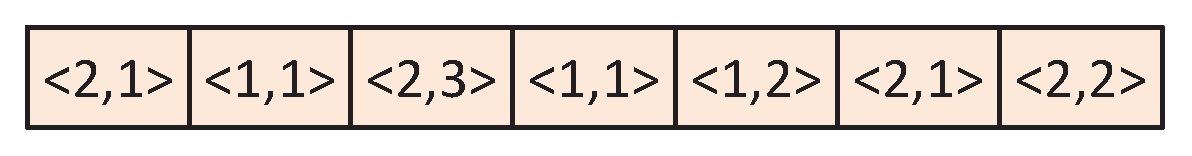
\includegraphics[scale=0.35]{chromo.eps}
	\end{center}
	\vspace{-0.2in}
		\caption{Example of a chromosome}
	\label{fig:chromosome}
\end{figure}
\vspace{-0.1in}

\subsubsection{Initial Population} In a genetic algorithm, the initial population consists of a group of individuals (or chromosomes),
where each of them
%which
represents a possible solution of the problem.
A chromosome is composed of several genes that are usually
represented by a random number, or a word or sentence over an
alphabet, or a bit. We use ``integer coding''~\cite{Goldberg} to represent a gene,
i.e. each gene is represented by a pair of non-negative integers. Fig. \ref{fig:chromosome} gives an example of a chromosome. % used in our algorithm.
In a chromosome, any gene $q$ is represented as an integer pair $\langle i,j\rangle$, if  the $q^{th}$ ($q=1\ldots n$) task (in $\Gamma$) is
assigned to core $\rho_{i,j}$ ($i=1\ldots m$, $j=1\ldots k_i$) (in $\Omega$). The number of genes in a chromosome is equal to $n$.
In  Fig. \ref{fig:chromosome}, the values of $m, k_i, \text{and } n$ are chosen as $2, 3, \text{and } 7$ respectively.



\subsubsection{Fitness Value} Each chromosome is assigned a \emph{fitness value} which determines the effectiveness of the solution
to the given problem. In our algorithm, the fitness value of a chromosome determines whether the corresponding task allocation
satisfies the constraints  in Eq. \ref{eq:ilp}, and how effectively
the task allocation minimizes the
total energy consumption.
%
%
%
%Let, $\Lambda$ be a large integer, $\kappa$, and $\nu$ be two constants.
%Eq. \ref{eq:fitness} represents the fitness function which is used to evaluate the chromosomes.
%The  fitness sub-function ($Fitness_{power}$, Eq. \ref{eq:fitness-p}) is used to evaluate the fitness of the chromosome in terms of minimizing the
%overall power consumption of the system.
%Whereas, fitness sub-function ($Fitness_{temp}$, Eq. \ref{eq:fitness-t}) is used to evaluate the fitness of the chromosome in terms of minimizing the
%overall temperature of the system.
%In this paper, our objective is to minimize the total power consumption while satisfying the maximum temperature constraints.
%So, we choose  $\kappa=1$, and $\nu=0$. Thus, a higher fitness value of a chromosome corresponds to an allocation strategy which results in
%lower total power consumption without violating the maximum temperature constraints.
%
Eq. \ref{eq:fitness-p} represents the fitness function of our genetic algorithm, which minimizes the
overall energy consumption of the system while satisfying the maximum temperature constraints.
If the allocation strategy corresponding to a chromosome violates Eq. \ref{eq:ilp}, then the penalty of the chromosome is
proportional to the frequency of the core
%chromosome is penalized
%proportionally to the speed assignment of the core
which violates  Eq. \ref{eq:ilp} (i.e. $\Lambda \times f_{i,j}$, where
$\Lambda$ is a large integer).
%where the violation happens (Eq. \ref{eq:penalize}).
Thus, a higher fitness value of a chromosome corresponds to an allocation strategy that results in
a lower total energy consumption without violating the maximum temperature constraints.


%\begin{equation}\label{eq:fitness}
%Fitness = \kappa * Fitness_{power} ~+~ \nu * Fitness_{temp}
%\end{equation}

\vspace{-0.2in}

\begin{subequations} \label{eq:fitness-p}
	\begin{equation}
	Fitness = E_{max} - E_{chromo}
	\end{equation}

\vspace{-0.2in}

	\begin{equation}
		E_{max} = P \sum_{i=1}^{m} \sum_{j=1}^{k_i} \Phi_{i,j}(f_{i,j}=f^{max}_{i,j})  %~( \text{when} ~~ f_{i,j}=f^{max}_{i} )
	\end{equation}

\vspace{-0.2in}

	\begin{equation}  \label{eq:penalize}
	\begin{split}
		&E_{chromo} = P \sum_{i=1}^{m} \sum_{j=1}^{k_i} \Phi^{'}_{i,j}(f_{i,j}) \\
		&\quad %\left(
		\text{\small where,  }
		 \Phi^{'}_{i,j}(f_{i,j}) = ~ \left\{ \begin{array}{ll}
		0 & \text{\small If $\rho_{i,j}$ is inactive} \\
		\Phi_{i,j}(f_{i,j}) & \text{\small If Eq. \ref{eq:ilp} is satisfied} \\
		\Lambda \times f_{i,j} & \text{\small Otherwise} \end{array}\right. %\right)
		\end{split}
	\end{equation}
\end{subequations}

\vspace{-0.1in}

%\begin{subequations} \label{eq:fitness-t}
%	\begin{equation}
%	Fitness_{temp} = Temp_{max} - Temp_{chromo}
%	\end{equation}
%
%	\begin{equation}
%		Temp_{max} = \sum_{i=1}^{m} \sum_{j=1}^{k} T^{max}_{i,j}
%	\end{equation}
%
%	\begin{equation}
%	\begin{split}
%		&~~Temp_{chromo} = \sum_{i=1}^{m} \sum_{j=1}^{k} T_{i,j} \\
%		&\quad \left( \text{where} ~~ T_{i,j} = \left\{ \begin{array}{ll}
%		T^*_{i,j} & \text{If Eq. \ref{eq:ilp} satisfies} \\
%		\Lambda . T^*_{i,j} & \text{Otherwise} \end{array}\right. \right)
%		\end{split}
%	\end{equation}
%\end{subequations}

\subsubsection{Crossover and Mutation} Crossover and Mutation are two genetic operators which are applied on the chromosomes
to produce new offsprings, hopefully with higher fitness values~\cite{Goldberg}.
\emph{Top-mate} selection procedure is used to select chromosomes for \emph{two-point crossover} \cite{Goldberg}, where the first chromosome for crossover is selected based on the order of fitness value and the second chromosome is selected randomly from all the chromosomes. In this type of
crossover, the genes between the two randomly chosen points of the selected chromosomes are interchanged with each other.
An example of a \emph{two-point crossover} %operation
is given in Fig. \ref{fig:crossover}.

\begin{figure}[h]
	\begin{center}
	%\vspace{-0.1in}
		\includegraphics[scale=0.35]{crossover.eps}
	\end{center}
	%\vspace{-0.2in}
		\caption{Example of a two-point crossover}
	\label{fig:crossover}
		%\vspace{-0.1in}
\end{figure}


Mutation %operator
is applied on the chromosomes to bring diversity in the population. The main objective of mutation
is to avoid losing useful information in the process of evolution \cite{Goldberg}. This also helps to improve the local search performance
of the genetic algorithm. \emph{Two-point mutation} is applied to a randomly selected chromosome. In this operation, the genes between
the two randomly chosen points of the chromosome are assigned new values. Fig. \ref{fig:mutation} gives an example of  \emph{two-point mutation}. % operation.

\begin{figure}[h]
	\begin{center}
	%	\vspace{-0.1in}
		\includegraphics[scale=0.35]{mutation.eps}
	\end{center}
		%\vspace{-0.2in}
		\caption{Example of a two-point mutation}
	\label{fig:mutation}
	%	\vspace{-0.2in}
\end{figure}


\subsubsection{Elitism and Regeneration} To ensure that the best fitness value of the next generation is not worse than that of the current generation,
a fixed number, MAX$^{elite}$, of best chromosomes are directly copied to the next generation. This operation is called \emph{elitism} \cite{Goldberg}.
The remaining population of the next generation are generated using crossover and mutation operators.


\subsubsection{Termination} The algorithm terminates when a fixed number, MAX$^{gen}$, of generations
%(denoted by MAX$^{gen}$)
have been computed, or the algorithm converges, i.e. the best fitness value of the population has not changed for a fixed number
of generations.

The pseudocode of the Genetic Algorithm (GA) based partitioning approach is given in Algorithm \ref{algo:ga}.

\begin{algorithm}
\caption{Genetic Algorithm Based Partitioning Approach} \label{algo:ga}
\footnotesize
\begin{algorithmic}[1]
\STATE Randomly generate the initial population
\STATE generation $\leftarrow$ 1
\WHILE {generation $\leq$ MAX$^{gen}$}
\STATE Compute fitness of the chromosomes using Eq. \ref{eq:fitness-p}
\STATE Rank the population based on the fitness value
\STATE Copy MAX$^{elite}$ best chromosomes to next generation, ties can be broken randomly
\STATE Generate remaining population using crossover
\STATE Mutate newly generated chromosomes
\IF {algorithm converged}
\STATE break
\ENDIF
\STATE generation  $\leftarrow$ generation  + 1
\ENDWHILE
\PRINT The total energy consumption, the allocation of tasks to cores, and the active/inactive states of cores that
correspond to the chromosome with the best fitness value (Ties are broken randomly)
\end{algorithmic}
\end{algorithm}

\vspace{-0.1in}

\subsection{Min-Core Worst-Fit Partitioning Heuristic}

In this partitioning heuristic, a task is allocated to a core according to  the
\emph{worst-fit} scheduling strategy, i.e.,
the algorithm always chooses a core with the maximum remaining capacity to assign the next task \cite{Langen09}, \cite{Aydin03}.
However,  \emph{worst-fit} scheduling only solves a part of the problem, i.e. it gives the allocation strategy.
%The problem of finding the minimum number of active cores to minimize the total power consumption remains unaddressed
%for the \emph{worst-fit} scheduling.
In order to find the optimal number of active cores,
we need to explore applying the allocation strategy to a variable number of available cores \cite{Langen09},
and thus identifying the optimal number of active cores needed to
%which
satisfy  the constraints in Eq.~\ref{eq:ilp}.
This motivates our Min-core Worst-fit partitioning (MW) heuristic described in Algorithm \ref{algo:mw}.
%we calculate the total power consumption without violating the
%constraints in Eq. \ref{eq:ilp} using a variable number of total available processors.


%The pseudocode of the Min-Core Worst-Fit Scheduling Heuristic (MW heuristic) is given
In Algorithm \ref{algo:mw},
the set of multiprocessors are sorted in decreasing order based on their respective performance coefficients.
The algorithm sequentially decreases the number of cores used in the worst-fit scheduling strategy (Lines \ref{for1}-\ref{for2}).
The process of decrementing the number of available cores stops, when the set of real-time tasks cannot be successfully scheduled using
the current number of active cores (Line \ref{stop}). % or the terminating conditions of the \emph{for} loops are satisfied.
Lines \ref{worst-start} to \ref{worst-end} give the pseudocode for worst-fit scheduling strategy using a fixed number of cores
(represented by the variable \emph{used cores} in Line \ref{core}).
The remaining capacities of all available cores are stored in a \emph{heap} data-structure (Line \ref{heap}).
A new task is allocated to a core with the maximum remaining capacity
that can successfully execute the task while satisfying the constraints in Eqs. \ref{eq:ilp}a and d (Lines \ref{allocation} to \ref{end-allo}).
It is possible that a core has a sufficient remaining capacity to execute a task, but its maximum temperature constraint
is violated. In such a circumstance, the algorithm tries to identify the next core from the heap which can successfully accommodate the task
while satisfying the temperature constraint (Lines \ref{inner-if} to \ref{end-inner}).
The total energy consumption of the system for a successful allocation strategy is computed in Line \ref{tpower}.
The information about a successful allocation strategy is stored in a stack (Line \ref{stack}), where
each element of the stack represents a tuple of the allocation strategy,  the
number of cores used in the allocation strategy, and the total energy consumption of the allocation strategy (Line \ref{triplet}).
%a tuple of three different variables (Line \ref{triplet}).
Finally, the element in the stack corresponding to the allocation strategy which results in the minimum total energy consumption
while satisfying the maximum temperature constraints is the output of the MW heuristic (Line \ref{out2} to \ref{out1}).
In case of a tie, the algorithm chooses an assignment strategy with the least number of active cores.
% The complexity of the algorithm is dominated by the three \emph{for} loops (Lines \ref{for1}, \ref{for2}, \ref{worst-start}), the \emph{while} loop (Line \ref{while}), and the thermal model used to estimate the maximum temperature of a core. The number of nodes in the \emph{heap} is bounded by the number of available cores in the worst-fit scheduling strategy. Using the HIT model, the maximum temperature of a core can be calculated in a constant time using Eq. \ref{eq:peak1}. However, using the HDT model, the estimation of the maximum temperature of a core takes $O(k^{2.38})$ time, if the number of cores ($k$) and the number of sinks ($h$)  in a multiprocessor unit satisfy the relation $k\in\Theta(h)$ and the inverse of $[A]_{k+h,k+h}$ is calculated using Coppersmith Winograd algorithm \cite{Coppersmith}. Thus, the time complexity of the MW heuristic using HIT and HDT model are $O( n( mk. \log (mk) )^2)$ and %$O( n( mk^{1.69}. \sqrt{\log (mk)} )^4)$ $O( n(mk^{1.69})^{4}. (\log (mk) )^2)$respectively, where $n$ is the number of tasks and $m$ is the number of multiprocessor units.

\begin{algorithm}
\caption{Min-Core Worst-Fit Partitioning Heuristic} \label{algo:mw}
\footnotesize
\begin{algorithmic}[1]
\REQUIRE $\Omega = \{\rho_1, \rho_2,\cdots, \rho_m\}$, a set of interconnected heterogeneous multiprocessor units
 sorted in decreasing order based on their respective performance coefficient $\alpha_i (i=1\ldots m)$.
 $\Gamma = \{\tau_1, \tau_2, \cdots, \tau_n\}$, a set of independent periodic real-time tasks.
%\ENSURE $\Omega = \{\rho_1, \rho_2,\cdots, \rho_m\}$ is sorted in decreasing order based on their performance coefficient $\alpha_i (i=1\ldots m)$
\FOR{$i = m \to 1$} \label{for1}
	\STATE Number of available cores in $\rho_l$ is $k_l, ~ (l=1 \ldots i-1)$
	\FOR{$j = k_i \to 1$} \label{for2}
		\STATE Number of available cores in $\rho_i$ is $j$
		\STATE Construct a \emph{heap} $\mathcal{H}$ of all available cores based on their remaining capacities, $\alpha_i \bar{U}_{i,j}$, where $\bar{U}_{i,j}$ is initialized to $1.0$ \label{heap}
		%\STATE Heapify the available cores based on their maximum available capacity of all available cores in a \emph{heap}, $\mathcal{H}$
		\FOR{$q = 1 \to n$} \label{worst-start}
			\IF{Allocating task $\tau_q$ to the core at the root of \emph{heap} $\mathcal{H}$ satisfies Eqs. \ref{eq:ilp}a and d} \label{allocation}
				\STATE Allocate task $\tau_q$ to the core at the root of  \emph{heap} $\mathcal{H}$
\STATE Change the core's remaining capacity $\alpha_i \bar{U}_{i,j}$ accordingly, where $\bar{U}_{i,j}$ is updated as $\bar{U}_{i,j} = \bar{U}_{i,j} - \frac{u_q}{\alpha_i}$
				\STATE \label{end-allo} Update  $\mathcal{H}$
			\ELSE
				\STATE Remove the root of  $\mathcal{H}$ \label{inner-if}
				\WHILE{$\mathcal{H} \neq $ empty} \label{while}
					\IF{Allocating task $\tau_q$ to the core at the root of \emph{heap} $\mathcal{H}$ satisfies Eqs. \ref{eq:ilp}a and d}
					\STATE Allocate task $\tau_q$ to the core at the root of  \emph{heap} $\mathcal{H}$
\STATE Change the core's remaining capacity $\alpha_i \bar{U}_{i,j}$ accordingly, where $\bar{U}_{i,j}$ is updated as $\bar{U}_{i,j} = \bar{U}_{i,j} - \frac{u_q}{\alpha_i}$
				\STATE \label{end-allo1} Update  $\mathcal{H}$

					\STATE break
					\ELSE
					\STATE Remove the root of  $\mathcal{H}$
					\ENDIF
				\ENDWHILE  \label{end-inner}
				\IF{$\mathcal{H} =$ empty} \label{stop}
					\STATE Insufficient number of available cores to schedule $\Gamma$
					\STATE Goto Line \ref{out2}
				\ENDIF
			\ENDIF
		\ENDFOR \label{worst-end}
		\STATE total energy $\leftarrow$ total energy consumption for this allocation strategy (using Eq. \ref{eq:power}) \label{tpower}
		%\STATE total number of available cores used in this allocation strategy
		\STATE \label{core} used cores $\leftarrow \sum_{l=1}^{i}k_l + j$
		\STATE  \label{triplet} $\mathcal{E}$ $\leftarrow$  (total energy, used cores, allocation strategy)
		%\STATE According to this allocation strategy, find the power consumption of each core using Eq. \ref{eq:power}
		\STATE \label{stack} push ($\mathcal{E}$) in stack $\mathcal{S}$
	\ENDFOR
\ENDFOR
\STATE \label{out2}  $\mathcal{E}$ $\leftarrow$ element in   $\mathcal{S}$ with the minimum total energy consumption
\PRINT  The total energy consumption, the allocation  strategy, and the number of active cores corresponding to  $\mathcal{E}$  \label{out1}
\end{algorithmic}
\end{algorithm}


\subsection{Hybrid Worst-Fit Genetic Algorithm} %Based Approach}

%In order
To improve the performances of both GA approach (Alg.~\ref{algo:ga}) and MW heuristic (Alg. \ref{algo:mw}),
we present Hybrid Worst-fit Genetic Algorithm (HyWGA).
HyWGA integrates the quickness of MW heuristic to generate a potential solution with the computational capability
of GA based approaches. % to improve the fitness value of a chromosome.
Thus, instead of randomly generating all the chromosomes of the initial
population, HyWGA modifies the initial population by including a chromosome which represents a solution of the MW heuristic.
The pseudocode of HyWGA is given in Algorithm \ref{algo:hywga}.

A balanced allocation of tasks based on the available capacity of cores often does not result in the lowest overall energy consumption due to the heterogeneity of multiprocessors. However, such bin packing techniques combined with the optimal number of active cores (similar to MW heuristic)
will result in  potential solutions for the energy-aware partitioning problem. Such potential solutions can also be included in the initial population
of the GA approach for improving its performance.
Investigation of such strategies %for the energy-optimal partitioning problem
is a future work.


\begin{algorithm}
\caption{Hybrid Worst-Fit Genetic Algorithm} \label{algo:hywga}
\footnotesize
\begin{algorithmic}[1]
\STATE Encode a chromosome which corresponds to the solution generated by Algorithm \ref{algo:mw}
\STATE Randomly generate the rest of the initial population
\STATE Call Algorithm \ref{algo:ga} on this initial population
\end{algorithmic}
\end{algorithm}
\vspace{-0.2in}


\section{Results and Discussion}

In this section, we present the simulation and analyze the simulation results
to compare the performance of the algorithms under both HIT and HDT thermal models.
The maximum allowed operating temperature of a core and the ambient temperature of the system are assumed to
be  $65^\circ C$ and $0^\circ C$ respectively. The task hyper-period $P$ is 1000 seconds.
The crossover and mutation rates for genetic algorithms are selected as 85\% and 0.5\% respectively. The value of
MAX$^{elite}$ is chosen as 1\% of the population size.

\subsection{Results using Heat-Independent  Thermal Model}

We assume a set of $8$ interconnected heterogeneous multiprocessor units (i.e. $m=8$), and each multiprocessor unit  is
assumed to have $8$ identical cores ($k_i=8, i=1 \ldots m$).
%In our model, we assume each core has discrete frequencies, i.e. the
%operating frequency of each core is in the range of $[f^{min}_i , f^{max}_i]$ ($i=1\ldots m$) with a step size of $0.05$,
%where $f^{min}_i = 50\% f^{max}_i$.
%The maximum allowed operating temperature of a core is assumed to be $70^\circ C$.
%We generated $12$
Twelve different periodic real-time task sets are generated by changing the values of $U_{tot}$ and the number of tasks ($n$).
The task sets for a given value of $U_{tot}$ were generated using normal distribution while selecting $n$ as $100, 150, 200,$ and $300$ respectively.
The values of $U_{tot}$ were chosen as  $20, 35,$ and $45$ respectively.
The size of the initial population, and the maximum number of generations for the genetic algorithms are selected as 2000, and 10,000 respectively.
%We have used a population size of 200 chromosomes , and heuristics ran for a maximum of 10,000 generations.
%The crossover and mutation rates for these heuristics were selected as 85\% and 0.5\% respectively. The value of
%MAX$^{elite}$ was chosen as 1\% of the population size, i.e. 20 chromosomes.
The parameters used in the simulation are  given in Table \ref{tab:simple}\footnote{It is assumed that $f_i^{min} = 0.5f_i^{max}$.} \cite{Quan10}, \cite{Leping10}, \cite{Chaturvedi10}.


\vspace{-0.1in}
\begin{table}[!h!tbs]
\caption{Simulation Parameters using HIT model}
\vspace{-0.1in}
\begin{center}
        \begin{tabular}{|c|c|c|c|c|c|c|c|c|}
        %\hline & & & & & & &  \\[-1.2ex]
        \hline
        $\rho_i$ & $f^{max}_i$ & $\gamma_i$ & $\delta_i$ & $\chi_i$ & $R_i$ & $C_i$ & $\alpha_i$  \\[0.5ex]
        \hline
        \hline $\rho_1$ & 3.3 & 20.5060 & 0.1666 & 3.656 & 0.282 & 340 & 2.152 \\
        \hline $\rho_2$ & 3.4 & 5.0187 & 0.1942 & 2.138 & 0.487 & 295 & 1.666 \\
        \hline $\rho_3$ & 3.3 & 12.7880 & 0.2043 & 3.645 & 0.288 & 320 & 1.148 \\
        \hline $\rho_4$ & 3.0 & 15.6262 & 0.1942 & 4.556 & 0.238 & 320 & 1.044 \\
        \hline $\rho_5$ & 3.2 & 20.6393 & 0.1574 & 3.204 & 0.278 & 295 & 0.869 \\
        \hline $\rho_6$ & 3.1 & 11.9759 & 0.1586 & 2.719 & 0.480 & 255 & 0.540 \\
        \hline $\rho_7$ & 3.0 & 10.3490 & 0.1124 & 2.074 & 0.661 & 335 & 0.348 \\
        \hline $\rho_8$ & 2.6 & 13.1568 & 0.1754 & 2.332 & 0.680 & 380 & 0.340 \\
        \hline
        \end{tabular}
\vspace{-0.1in}
\label{tab:simple}
\end{center}
\end{table}
\vspace{-0.1in}



\emph{Traditional power models} assume fixed static power
consumption of a core~\cite{Chen09}.
%(i.e. the leakage current is fixed) \cite{Chen09}.
For comparison purpose, we modified the MW heuristic to use the \emph{traditional power model}, and denote it as M-MW heuristic.
The estimated temperature and power of a core using the M-MW heuristic may not be accurate due to its ineffectiveness in incorporating the impact of both temperature and voltage on the leakage current.
%the dynamic nature of leakage current.
Thus, the actual temperature and power of a core may be significantly higher than its estimated value, which may result in violation of maximum temperature constraints and very high energy consumption, as observed in our simulation (Figs. \ref{fig:l20}-\ref{fig:l45}).
%For fair comparison, the power consumption of the allocation strategy for the M-MW heuristic (reported in Fig. \ref{fig:simple}) is calculated using the proposed power and HIT models.



The performance of the algorithms using the HIT model are compared in Fig. \ref{fig:simple}.
The total energy consumption of the algorithms under different task sets are shown in Figs.~\ref{fig:l20}-\ref{fig:l45}.
Overall, HyWGA is most effective in generating an allocation strategy which results in the minimum energy consumption.
In our experiments, HyWGA reduces the total energy consumption by 5\% to 11\% as compared to the MW heuristic.
The total number of active cores used by the algorithms in their respective minimum-energy allocation strategies
%which results in minimum energy consumption
%under different task sets
are compared in Figs.~\ref{fig:c20}-\ref{fig:c45}.
%In Fig. \ref{fig:c20}, minimum energy allocation strategy generated by GA uses a high number of active cores.
%This is primarily due to the randomness in the  generation of the entire initial population.
In Figs. \ref{fig:c35} and \ref{fig:c45}, the minimum-energy allocation strategies
generated by HyWGA use higher numbers of active cores than those generated by MW heuristic.
The MW heuristic explores \emph{worst-fit} scheduling strategy using a variable number of active cores. However, MW heuristic needs  a set
of interconnected heterogeneous multiprocessor units which is sorted in descending order based on their respective performance coefficients.
Thus, MW heuristic is biased in favor of a low number of cores with high performance coefficients. This kind of selection strategy is more likely to identify
a core with lower performance coefficient as an inactive core compared to a high performance coefficient core.
This feature of MW heuristic prohibits it to explore an allocation strategy which can combine a mixture of cores with different
performance coefficients.
By leveraging a genetic algorithm and its computational effectiveness, HyWGA addresses this drawback, where it explores different task allocations without any biases in selection of the active cores.
A comparison of the total energy consumption by using a different number of active cores in MW heuristic (when $U_{tot}=20$ and $n=150$)
is shown in Fig. \ref{fig:s-cores}. It can be observed that there are several extreme points in Fig. \ref{fig:s-cores}.
Thus, it is important to explore all the values of the number of active cores to identify the minimum-energy allocation strategy. In Fig. \ref{fig:s-cores},
using 10 or fewer cores in the allocation strategy cannot satisfy the constraints in Eq. \ref{eq:ilp}.

\begin{figure*}[!t]
%\vspace{-0.12in}
	\begin{center}
		\subfigure[Total Energy Consumption for $U_{tot}=20$]{\label{fig:l20}\includegraphics[scale=0.35]{simple_1.eps}}
		\subfigure[Total Energy Consumption for $U_{tot}=35$]{\label{fig:l35}\includegraphics[scale=0.35]{simple_2.eps}}
		\subfigure[Total Energy Consumption for $U_{tot}=45$]{\label{fig:l45}\includegraphics[scale=0.35]{simple_3.eps}}
		\subfigure[Total Number of Active cores for $U_{tot}=20$]{\label{fig:c20}\includegraphics[scale=0.35]{simple_4.eps}}
		\subfigure[Total Number of Active cores for $U_{tot}=35$]{\label{fig:c35}\includegraphics[scale=0.35]{simple_5.eps}}
		\subfigure[Total Number of Active cores for $U_{tot}=45$]{\label{fig:c45}\includegraphics[scale=0.35]{simple_6.eps}}
		\subfigure[Impact of ordering the tasks ($U_{tot}=45$)]{\label{fig:s-order}\includegraphics[scale=0.35]{simple_7.eps}}
		\subfigure[Active Cores vs. Total Energy Consumption]{\label{fig:s-cores}\includegraphics[scale=0.36]{new_simple_8.eps}}
		\subfigure[Maximum Fitness vs. Generations]{\label{fig:s-genetic}\includegraphics[scale=0.35]{simple_9.eps}}
	\end{center}
	\vspace{-0.12in}
		\caption{Results using Heat-Independent  Thermal Model}
	\label{fig:simple}
%\vspace{-0.15in}
\end{figure*}

The impact of sorting tasks (based on their utilizations) on the performance of the algorithms is shown in Fig. \ref{fig:s-order}.
If the algorithm uses a task set which has been sorted in decreasing order of task utilizations, then the name of the algorithm is appended with $-D$ (e.g. MW-D)
in the legend of Fig. \ref{fig:s-order}.
Similarly, we append $-A$ to the name of the algorithm in the legend of Fig. \ref{fig:s-order}, if it uses a task set which has been
sorted in ascending order of task utilizations (e.g. GA-A).
The MW heuristic has the best performance when a task set is sorted in a decreasing utilization order.
This observation verifies that the \emph{worst-fit} scheduling strategy has the best performance for \emph{bin-packing} problem, when the
items are sorted with decreasing sizes \cite{Aydin03}. Due to a similar reasoning, the performance of the MW heuristic is adversely affected
by sorting tasks in ascending order of their utilizations.
In our experiments, the total energy consumption
of the MW heuristic decreases by 0.2\% to 3\%, if task sets are sorted with decreasing task utilizations.
However, this improvement in performance due to ordering of task sets is %not observed
negligible
in GA and HyWGA approaches.


The maximum fitness value of each generation of the GA and HyWGA are compared in Fig. \ref{fig:s-genetic} (when $U_{tot}=35$ and $n=200$).
The maximum fitness value of the GA approach
converges quickly to its optimal value. On the other hand, the maximum fitness value of HyWGA approach increases %very
slowly from generation to generation, because the initial population's fitness value is  close to its optimal value.
Interestingly, randomness of initial population of GA approach sometimes results in an allocation strategy with the lowest energy consumption ($U_{tot}=45, n=100$).
This advantage adversely affects the performance of the GA algorithm when there are a high number of tasks with a low total utilization.
In this case, the randomness in GA approach causes its allocation strategy to use a high number of active cores (Fig. \ref{fig:c20}),
resulting in a higher total energy consumption. %, primarily due to the static power consumption of an active core.


\subsection{Results using Heat-Dependent Thermal Model}


We assume a set of $4$ interconnected heterogeneous multiprocessor units (i.e. $m=4$), and
%each multiprocessor unit  is assumed to have $4$ identical cores (i.e. $k=4$). We
assume the layout of the multiprocessor is $2\times 2$ with 2 sinks, i.e. each unit has $4$ identical cores ($k_i=4, i=1 \ldots m$)  \cite{Chantem10}, \cite{Fisher09}.
%We generated $6$
Six different periodic real-time task sets
are generated
by changing the values of $U_{tot}$ and the  number of tasks ($n$).
The task sets for a given value of $U_{tot}$ were generated using normal distribution while selecting $n$ as $100$ and $200$ respectively.
The values of $U_{tot}$ were chosen as  $5, 10,$ and $15$ respectively.
The size of the initial population, and the maximum number of generations for the genetic algorithms are selected as 200, and 500 respectively.
The parameters used in the simulation are given in Table~\ref{tab:complex}\footnote{It is assumed that $f_i^{min} = 0.5f_i^{max}$.}~\cite{Fisher09}. According to Eq. \ref{eq:complex_peak1}, the value of $A_{i,i}$ $(i=1\ldots4)$ in matrix A
can only be computed after the frequencies of cores have been determined.
These entries are left blank in Table \ref{tab:complex}.
%Thus, these entries are left blank in Table \ref{tab:complex}.



%\vspace{-0.1in}
\begin{table}[!h]  %!tbs]
\caption{Simulation Parameters using HDT model}
\vspace{-0.2in}
\centering
\label{tab:complex}
\subtable[Matrix A for $\rho_1$]{
	\begin{tabular}{ |c|c|c|c|c|c| }
	\hline
	 & 0.009 & 0.004 & 0.000 & 0.200 & 0.050 \\
	\hline 0.009 &  & 0.000 & 0.004 & 0.050 & 0.060 \\
	\hline 0.004 & 0.000 &  & 0.009 & 0.200 & 0.050 \\
	\hline 0.000 & 0.004 & 0.009 &  & 0.050 & 0.060 \\
	\hline 0.200 & 0.050 & 0.200 & 0.050 & -1.725 & 0.300 \\
	\hline 0.050 & 0.060 & 0.050 & 0.060 & 0.300 & -1.445 \\
	\hline
	\end{tabular}
}
\subtable[Matrix A for $\rho_2$]{
	\begin{tabular}{ |c|c|c|c|c|c| }
	\hline
	 & 0.025 & 0.007 & 0.020 & 0.500 & 0.050 \\
	\hline 0.025 &  & 0.020 & 0.007 & 0.050 & 0.200 \\
	\hline 0.007 & 0.020 &  & 0.025 & 0.500 & 0.050 \\
	\hline 0.020 & 0.007 & 0.025 &  & 0.050 & 0.200 \\
	\hline 0.500 & 0.050 & 0.500 & 0.050 & -2.925 & 0.900 \\
	\hline 0.050 & 0.200 & 0.050 & 0.200 & 0.900 & -2.325 \\
	\hline
	\end{tabular}
}
\subtable[Matrix A for $\rho_3$]{
	\begin{tabular}{ |c|c|c|c|c|c| }
	\hline
	 & 0.020 & 0.010 & 0.000 & 0.400 & 0.100 \\
	\hline 0.020 &  & 0.000 & 0.010 & 0.100 & 0.120 \\
	\hline 0.010 & 0.000 &  & 0.020 & 0.400 & 0.100 \\
	\hline 0.000 & 0.010 & 0.020 &  & 0.100 & 0.120 \\
	\hline 0.400 & 0.100 & 0.400 & 0.100 & -2.625 & 0.700 \\
	\hline 0.100 & 0.120 & 0.100 & 0.120 & 0.700 & -2.065 \\
	\hline
	\end{tabular}
}
\subtable[Matrix A for $\rho_4$]{
	\begin{tabular}{ |c|c|c|c|c|c| }
	\hline
	 & 0.013 & 0.007 & 0.004 & 0.300 & 0.050 \\
	\hline 0.013 &  & 0.004 & 0.007 & 0.080 & 0.090 \\
	\hline 0.007 & 0.004 &  & 0.013 & 0.300 & 0.080 \\
	\hline 0.004 & 0.007 & 0.013 &  & 0.080 & 0.090 \\
	\hline 0.300 & 0.080 & 0.300 & 0.080 & -2.085 & 0.400 \\
	\hline 0.080 & 0.090 & 0.080 & 0.090 & 0.400 & -1.665 \\
	\hline
	\end{tabular}
}
\subtable[Other Simulation Parameters]{
				\begin{tabular}{|c|c|c|c|c|c|}
        %\hline & & & & &  \\[-1.2ex]
        \hline
        $\rho_i$ & $f^{max}_i$ & $\gamma_i$ & $\delta_i$ & $\chi_i$  & $\alpha_i$  \\[0.5ex]
        \hline
        \hline $\rho_1$ & 2.2 & 0.10 & 0.002 & 1.0  & 2.152 \\
        \hline $\rho_2$ & 2.5 & 0.20 & 0.015 & 1.3  & 1.666 \\
        \hline $\rho_3$ & 2.0 & 0.18 & 0.010 & 2.2  & 1.044 \\
        \hline $\rho_4$ & 1.9 & 0.15 & 0.005 & 1.7  & 0.540 \\
        \hline
        \end{tabular}
}
\vspace{-0.2in}
\end{table}

%Thus, Figs. \ref{fig:l20}-\ref{fig:l45} compares the performance of the heuristics using different thermal model.

The HDT model captures the impact of heat transfer among different cores (Section \ref{sec:complex}).
However, this transfer of heat among different cores is not captured in the HIT model (Section \ref{sec:simple}).
Thus, when the heat transfer among cores is non-negligible, it is expected that the HDT model would result in a more accurate estimation of the core's temperature
%. This will
leading to a better estimation of
energy consumption of a core. Let us consider multiprocessor unit $\rho_2$ for scheduling a task set. Let the non-normalized frequencies of $\rho_{2,1}$, $\rho_{2,2}$,
$\rho_{2,3}$, and $\rho_{2,4}$ be 2, 1.9, 2.1, and 1.7 Ghz respectively. Accordingly to the HIT model, $T^*_{2,1}=53.9^\circ C$,  $T^*_{2,2}=46.1^\circ C$,
$T^*_{2,3}=62.7^\circ C$, and  $T^*_{2,4}=36.7^\circ C$. This is expected as a lower frequency in the HIT model results in a lower maximum temperature (Eq.~\ref{eq:peak1}).
%
%Thus we get, $\Phi_{2,1}=12.41$ Watt, $\Phi_{2,2}=10.61$ Watt, $\Phi_{2,3}=14.43$ Watt, and $\Phi_{2,4}=7.66$ Watt. So, the overall energy consumption of $\rho_2$ according to the HIT model is $45.11$ KJ.
%
However, there is heat transfer among cores. Applying the HDT model, the actual maximum temperatures of the cores with the same frequency assignment are,
$T^*_{2,1}=50.6^\circ C$,  $T^*_{2,2}=66.5^\circ C$, $T^*_{2,3}=53.5^\circ C$, and  $T^*_{2,4}=56.8^\circ C$.
These maximum temperature values reflect the impact of heat transfer among cores. For example, even if $\rho_{2,4}$ runs at a lower frequency,
it still has a high temperature due to thermal conductivity between the cores and sinks. A more critical problem is: this frequency assignment violates the
maximum temperature constraint for $\rho_{2,2}$, which fails to be detected by the HIT model.
%
%According to the HDT model, the values of $\Phi_{2,1}$, $\Phi_{2,2}$, $\Phi_{2,3}$, and $\Phi_{2,4}$ are 12.31 Watt, 11.19 Watt, 14.14 Watt, and 8.17 Watt. Thus, the total energy consumption of $\rho_2$ is actually 45.81 KJ.
%
This example demonstrates the importance of using an accurate model, i.e., the HDT model to capture the heat transfer among cores. An inaccurate model may lead to the violation of temperature constraints, resulting in reduced system reliability and performance in a long run.
Moreover, this inaccuracy can also result in inaccurate estimation of total energy consumption of the system, as observed in our simulation.


%If the maximum temperature constraints were not violated by the HIT model, then the estimated total energy consumption using HIT model is  within 1.6\% of its actual value (estimated using HDT model). We find this error bound to be less than 13\% in our experiments (Fig. \ref{fig:complex}). Therefore, in special scenarios when temperature constraints could be relaxed, there is a trade-off between the accuracy in the estimation of energy consumption vs. the speed of computation in these thermal models. Surprisingly, this error bound is less than 0.2\% for MW heuristic.



%
%In our experiments (Fig. \ref{fig:complex}), the estimation of energy consumption using HI model is within 13\% of the energy consumption calculated by HD model,
%assuming that the maximum temperature constraint was not violated by the HI model. Interestingly, in our experiments the error of estimation of MW-Ind heuristic
%is less than 0.2\% as compared with MW heuristic.



%The performance of the algorithms using the HDT model are compared in Fig. \ref{fig:complex}.
%%In Fig. \ref{fig:complex}, the legends MW-Ind, GA-Ind, and HyWGD-Ind represents the performance of MW, GA, and HyWGD heuristics using the HIT model.
%The total energy consumption of the algorithms under different task sets are shown in Figs. \ref{fig:l5}-\ref{fig:l15}.
%Overall, the HyWGA algorithm is the best in generating an allocation strategy which results in the minimum energy consumption.
%In our experiments, the HyWGA algorithm reduces the total energy consumption by up to 21\% as compared to the MW heuristic.
%%In Fig. \ref{fig:complex} we observe a trend similar to Fig. \ref{fig:simple}, i.e. increasing the number of active cores
%%may result in lower total energy consumption.
%The total number of active cores used by the algorithms in their respective minimum-energy allocation strategies
%are compared in Figs. \ref{fig:c5}-\ref{fig:c15}.
%Due to the randomness in the initial population of GA algorithm, the minimum-energy allocation strategy for a task set with $U_{tot}=5$ or $10$
%uses a higher number of active cores, resulting in a higher total energy consumption. % due to higher static power consumption.


The performance of the algorithms using HDT model are compared in Fig. \ref{fig:complex}.
In Fig. \ref{fig:complex}, the name of the algorithm is appended with -HIT, when the temperature was estimated using  HIT model.
Interestingly, the estimated total energy consumption using HIT model is  within 1.6\% of the value estimated using HDT model.
Therefore, in special scenarios when temperature constraints could be relaxed, there is a trade-off between the accuracy in the estimation of energy consumption vs. the speed of computation of the thermal model.
The total energy consumption of the algorithms under different task sets are shown in Figs. \ref{fig:l5}-\ref{fig:l15}.
Overall, HyWGA approach is the best in generating an allocation strategy which results in the minimum energy consumption.
In our experiments, HyWGA reduces the total energy consumption by up to 21\% as compared to the MW heuristic.
%In Fig. \ref{fig:complex} we observe a trend similar to Fig. \ref{fig:simple}, i.e. increasing the number of active cores
%may result in lower total energy consumption.
The total number of active cores used by the algorithms in their respective minimum-energy allocation strategies
are compared in Figs.~\ref{fig:c5}-\ref{fig:c15}.
Due to the randomness in the initial population of GA algorithm, the minimum-energy allocation strategy for a task set with $U_{tot}=5$ or $10$
uses a higher than optimal number of active cores, resulting in a higher total energy consumption. % due to higher static power consumption.



%In order to make a fair comparison between the two thermal models, we ensure that running the cores with a speed corresponding to
%the minimum energy allocation strategy generated using HI model, does not really violate the maximum temperature constraints (using HI model).
%The execution time of heuristics using HD model is much slower than that using HI model. This is primarily due to the complexity involved in
%solving Eq. \ref{eq:complex_peak1}. So, there is a trade-off between computational efficiency and the use of more realistic model thermal model, HD model.
%We analyze this trade-off in Figs. \ref{fig:l20}-\ref{fig:l45}.


%The minimum energy consumption given by MW-Ind, GA-Ind, and HyWGA-Ind
%are close estimates of the actual minimum energy consumption corresponding to the MW, GA, and HyWGA heuristics respectively, at the cost of
%much faster execution time.  For example, the execution times for allocation 100 tasks with $U_{tot}=100$ for MW, MW-Ind, GA, GA-Ind,
%HyWGA, and HyWGA-Ind heuristics on AMD Turion X2 TL-60 2Ghz processor are 42sec, 11sec,  x, x, 410sec, 6sec,

The impact of sorting a task set (based on task utilizations) on the performance of the algorithms is shown in Fig. \ref{fig:c-order}.
The legends used in Fig. \ref{fig:c-order} have similar meanings to those used in Fig. \ref{fig:s-order}. We observe that, due to the heat transfer among cores, the MW heuristic may not always have the best performance when tasks are sorted in decreasing order of their utilizations.
The maximum fitness value of each generation of the GA and HyWGA approaches are compared in Fig. \ref{fig:c-genetic} (when $U_{tot}=10$ and $n=100$).
A comparison of the total energy consumption by using a different number of active cores by MW heuristic (when $U_{tot}=10$ and $n=100$)
is shown in Fig. \ref{fig:c-cores}. In both of these figures, we observe a  trend similar to that in  Figs. \ref{fig:s-cores}-\ref{fig:s-genetic}.


\begin{figure*}[!t]
%\vspace{-0.12in}
	\begin{center}
		\subfigure[Total Energy Consumption for $U_{tot}=5$]{\label{fig:l5}\includegraphics[scale=0.35]{complex_1.eps}}
		\subfigure[Total Energy Consumption for $U_{tot}=10$]{\label{fig:l10}\includegraphics[scale=0.35]{complex_2.eps}}
		\subfigure[Total Energy Consumption for $U_{tot}=15$]{\label{fig:l15}\includegraphics[scale=0.35]{complex_3.eps}}
		\subfigure[Total Number of Active cores for $U_{tot}=5$]{\label{fig:c5}\includegraphics[scale=0.35]{complex_4.eps}}
		\subfigure[Total Number of Active cores for $U_{tot}=10$]{\label{fig:c10}\includegraphics[scale=0.35]{complex_5.eps}}
		\subfigure[Total Number of Active cores for $U_{tot}=15$]{\label{fig:c15}\includegraphics[scale=0.35]{complex_6.eps}}
		\subfigure[Impact of ordering the tasks ($U_{tot}=10$)]{\label{fig:c-order}\includegraphics[scale=0.35]{complex_7.eps}}
		\subfigure[Active Cores vs. Total Energy Consumption]{\label{fig:c-cores}\includegraphics[scale=0.45]{new_complex_8.eps}}
		\subfigure[Maximum Fitness vs. Generations]{\label{fig:c-genetic}\includegraphics[scale=0.35]{complex_9.eps}}
	\end{center}
	\vspace{-0.12in}
		\caption{Results using Heat-Dependent  Thermal Model}
	\label{fig:complex}
%\vspace{-0.15in}
\end{figure*}

\section{Conclusion}

%In this paper, we model the impact of leakage current on the static power consumption. The power equation is modeled to incorporate the impact of temperature and voltage on the leakage current of a processor.

This paper develops a genetic-algorithm based approach (HyWGA) to solve the thermal-constrained energy-aware partitioning problem for heterogeneous multi-core multiprocessor real-time systems.
Our solution is novel in that it considers a power model that captures not only the leakage power consumption, but also the impact of temperature and voltage on the leakage current of a processor. We have used two different thermal models to estimate the temperature of a processor with both negligible and non-negligible amount of heat transfer among cores and sinks of a multiprocessor system.

We present several algorithms to identify cores to be activated and to allocate tasks to cores so as to minimize
%optimal number of active cores, and the allocation strategy for a task set that minimizes
the total energy consumption while satisfying maximum temperature and deadline constraints. Extensive experimental simulations have been conducted to analyze the performance of the algorithms. From the analysis of experimental data, we observe that our HyWGA approach is most effective in minimizing the total energy consumption. It can minimize the total energy consumption by up to 11\% and 21\%, as compared to the %worst-fit based
MW heuristic, when using the HIT and HDT models respectively.

The off-line HyWGA approach developed in this paper is the first step towards solving the energy control problem for heterogeneous multi-core multiprocessor real-time systems. In the future, we will develop complementary and more efficient online strategies to handle practical issues like modeling inaccuracies of task execution times, power and thermal parameters, where task partitioning will be adapted according to the actual measurements of parameters.

%online scheduling strategies using actual worst case execution time of the tasks for simultaneously minimizing both the total energy consumption and the maximum temperature of the system.

%We would  modify the  fitness function of the genetic algorithm to incorporate such multi-objective scheduling. We would also like to investigate scheduling algorithms based on two-speed scheduling strategies  \cite{Quan10}, which would satisfy the maximum temperature constraint and also minimize the maximum temperature when the system may not reach  steady state condition during the interval $[0,P]$.

\bibliography{rtss}
\bibliographystyle{ieeetr}


%
%\begin{thebibliography}{00}
%\end{thebibliography}

\end{document}



